\chapter{Omisión de palabras}

Anteriormente se especificó que la base de datos de los préstamos serían únicamente palabras de contenido, y a partir de ellas se realizaron los análisis anteriores.  Al trabajar con las palabras de contenido se están restringiendo a todas las palabras que pueden ser catalogadas como préstamos (algunos artículos o pronombres de un determinado idioma se encuentran en los demás), sin embargo los resultados obtenidos han reflejado contextos históricos en los cuáles explicar las migraciones de palabras, por lo que las restricciones han ayudado a deducciones más claras. 

Por el momento ya no se tratara con la misma regularidad a la interpretación histórica de las migraciones, se centrara las siguientes partes en la forma en que se modifican los resultados al hacer diferentes restricciones en el conjunto de préstamos. 

Si se toman como verdadero al uso de un idioma sobre otro, discutido en capítulo 3,  del conjunto de palabras que conforman en uso de un idioma se propondrán diferentes reglas para restringir al conjunto y observar cómo es que cambian los datos del conjunto reducido por la restricción contra el conjunto original.  

Por ejemplo,  si la regla es omitir las palabras que comiencen con la letra C,  el conjunto original contendrá a todos los préstamos,  el conjunto reducido  no tendrá  préstamos cuya primer letra sea C y el conjunto de las restricciones serán todos los préstamos que empiecen con C. Una vez separados los conjuntos en cada uno se realizó el proceso de  la ecuación \ref{ec.fuso}, para obtener el uso.

Todas las reglas para las omisiones serán eliminando las palabras que comienzan con una determinada letra, en algunos casos se optó por hacer hasta cuatro omisiones con la intención de restringir cada vez más a los conjuntos.  Para una adecuada comparación del uso de un idioma sobre otro, se gráfico de manera continua y  en color negro al conjunto original,  mientras que puntos de dispersión de color rojo al conjunto reducido.


\newpage
\subsection{Inglés}

\begin{figure}[h!]
	\centering
	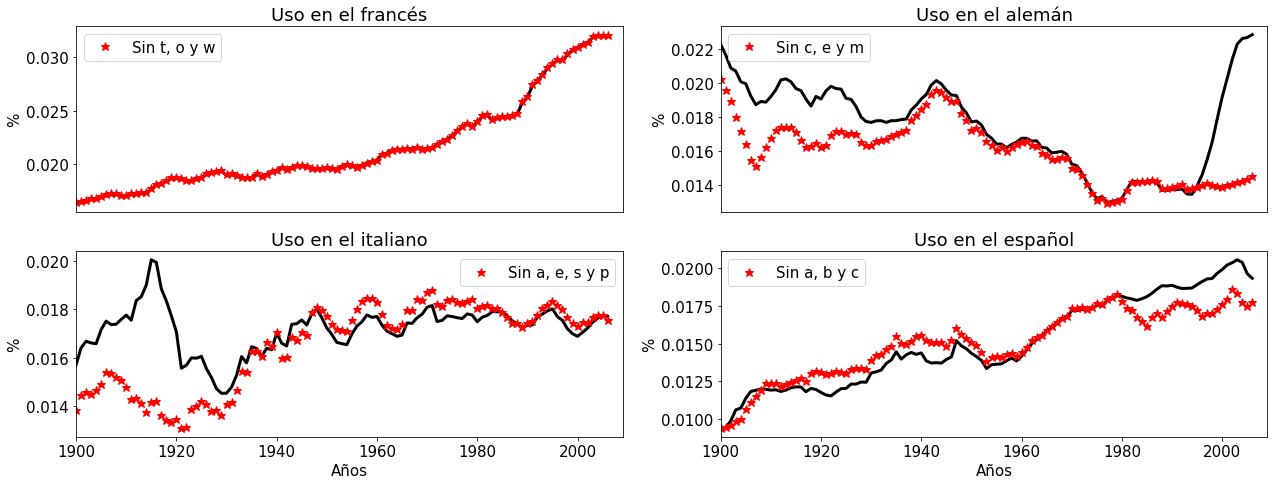
\includegraphics[scale=.375]{Cap_5/OM_EN.png}
	\label{fig.OM_EN}
	\caption{Omisiones del inglés en los demás}
\end{figure}



\newpage
\subsection{Francés}

\begin{figure}[h!]
	\centering
	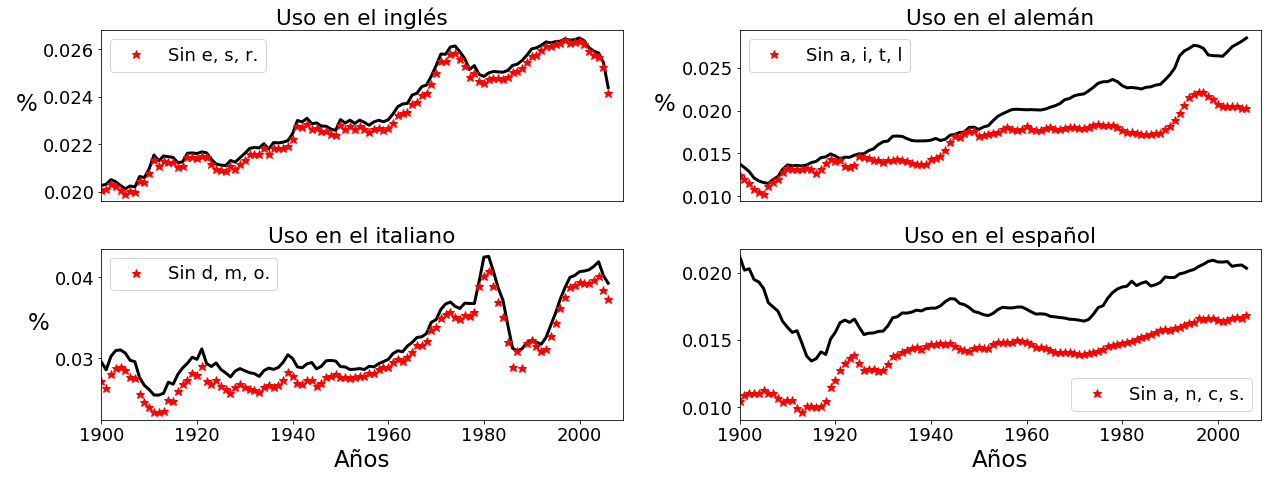
\includegraphics[scale=.375]{Cap_5/OM_FR.png}
	\label{fig.OM_FR}
	\caption{Omisiones del francés en los demás}
\end{figure}


\newpage
\subsection{Alemán}

\begin{figure}[h!]
	\centering
	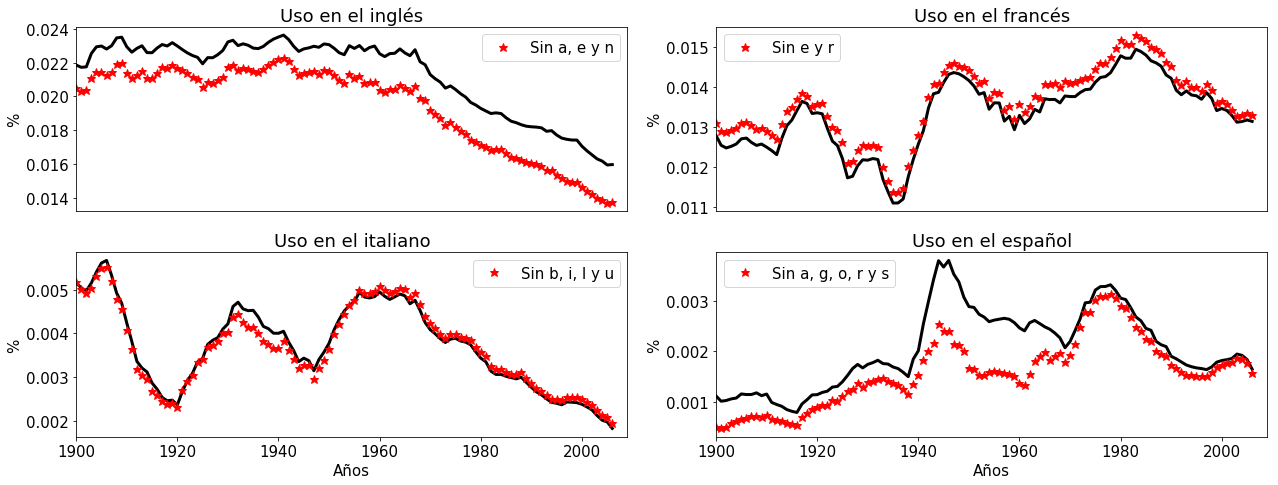
\includegraphics[scale=.375]{Cap_5/OM_GE.png}
	\label{fig.OM_GE}
	\caption{Omisiones del alemán en los demás}
\end{figure}


\newpage
\subsection{Italiano}

\begin{figure}[h!]
	\centering
	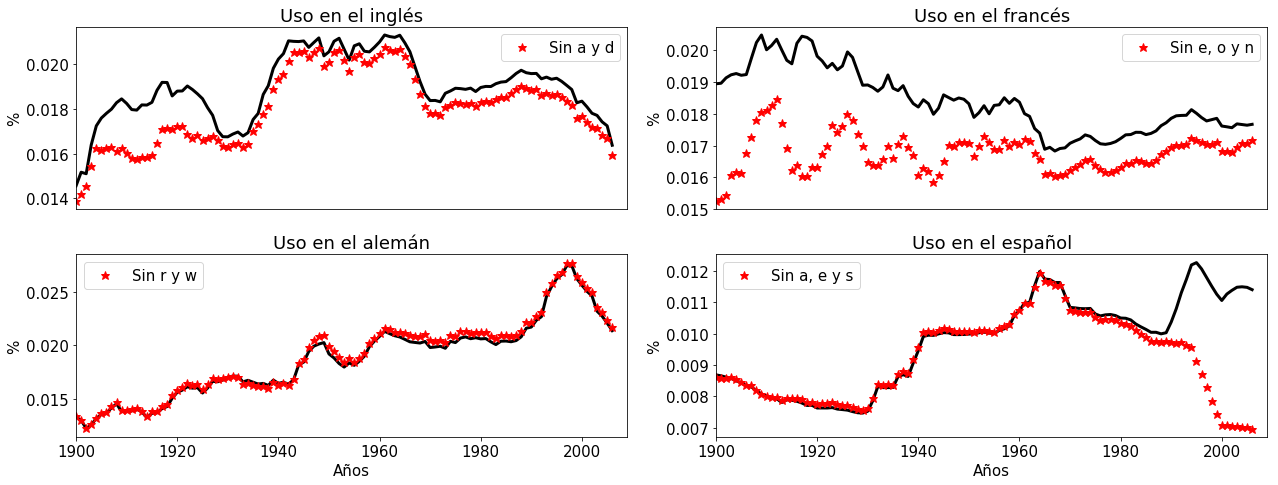
\includegraphics[scale=.375]{Cap_5/OM_IT.png}
	\label{fig.OM_IT}
	\caption{Omisiones del italiano en los demás}
\end{figure}


\newpage
\subsection{Español}

\begin{figure}[h!]
	\centering
	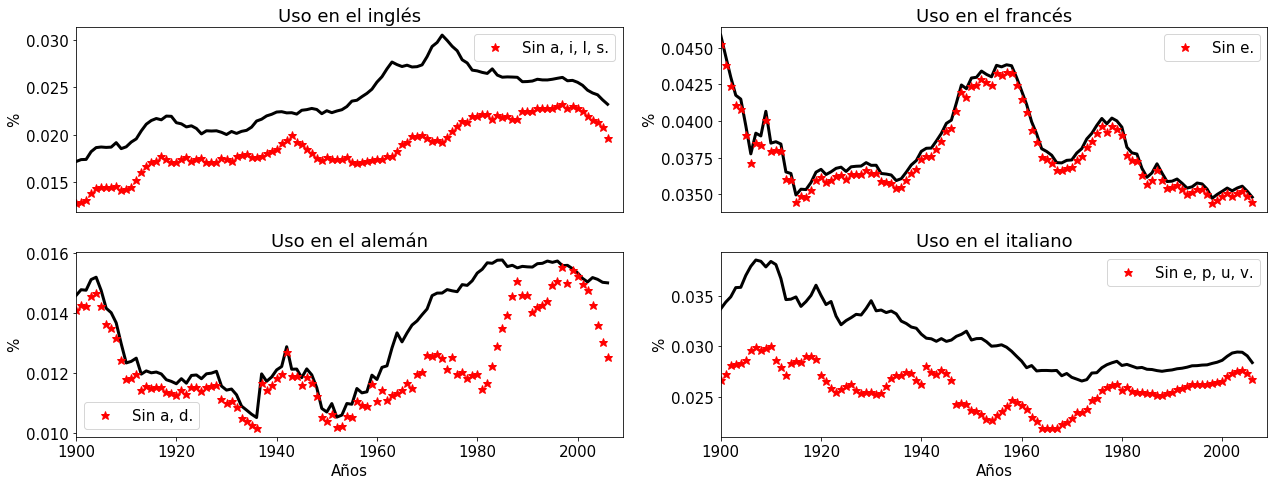
\includegraphics[scale=.375]{Cap_5/OM_SP.png}
	\label{fig.OM_SP}
	\caption{Omisiones del español en los demás}
\end{figure}
